\chapter{ABILITY SCORES}

\begin{multicols}{2}

\index{Ability Scores}All characters are represented by six ability scores; three physical and three mental.  The method \index{Ability Scores!Generation}for generating ability scores is determined by the GM.  

\paragraph{Method I - Traditional:}  Roll 3d6 in order of attributes: strength, dexterity, constitution, intelligence, wisdom, and charisma.

\paragraph{Method II - Contemporary:}  Roll 4d6 six times, dropping the lowest number, and assign as the player chooses.

\paragraph{Method III - New Age:}  Roll 4d4~+~2 six times and assign as the player chooses.

\paragraph{Method IV - Points System:}  Characters have 60~+~4d4 points to assign to their abilities (minimum 3 and maximum 18).  Each 10\% of exceptional strength costs 1 point.

\subparagraph{}Human characters will typically have a score between 3--18 with 9--11 being the typical average.  Non-human races have ability requirements; if the ability scores do not meet the requirement, the character cannot be that race.  A starting character won't have a single ability score above 18 with the exception of racial bonuses or exceptional strength provided the character is a warrior.

\section{STRENGTH}

\index{Strength}Strength (Str) represents raw muscle mass and is the most important ability score for warriors.  A warrior with strength of 18 can roll a d\% for exceptional strength.  An 18/61 is stronger than an 18/35.

\index{Melee Attack Modifier}\paragraph{Melee Attack Modifier:}  Modifies the character's ability to hit with a melee weapon or bow.  Refer to Weapons and Armor: Bows, for more information.

\index{Damage Modifier}\paragraph{Damage Modifier:}  This bonus is applied to the damage of melee weapons, hurled weapons, and bows, but never crossbows.  Refer to Weapons and Armor: Bows, for more information.

\index{Non-encumbered Weight}\paragraph{Non-Encumbered:} How much weight a character can carry on his person without feeling the effects of encumbrance (Refer to Encumbrance).

\index{Maximum Weight}\paragraph{Max Weight:}  The maximum amount of weight the character can carry on his person.  If a character carries more weight than they're allowed, they cannot move or act.

\index{Force Doors}\paragraph{Force Doors:}  The chance to force open a large or stuck door on a roll of 1d20.  If the number is equal to or less than the number the door is forced open.  Each attempt takes an amount of time determined by the GM and creates considerable noise.  The number in parentheses is the chance to force open a locked (magical or mundane) or barred door.  Retrying a failed roll is not possible.

\index{Bend Bars/Lift Portcullis}\paragraph{Bend Bars/Lift Portcullis:}  The chance to physically bend strong metal bars or lift a heavy portcullis.  Retrying a failed roll is not possible.

Bonuses and Penalties to Exceptional Strength Scores: If a character with exceptional strength receives a bonus or penalty to his strength score, whether permanent or temporary, from a spell, magic item or some other magical means, each point of bonus or penalty equates to one category increase or decrease in the character's exceptional strength, placing them in the middle of the next lowest or highest category.  This does not include racial modifiers for strength given while the character is created.

For each +1 bonus or $-1$ penalty, the results for exceptional strength are shown here:
18/01--50 will rise to 18/64 or drop to standard 18; 18/51--75 will rise to 18/83 or drop to 18/25; 18/76--90 will rise to 18/95 or drop to 18/64; 18/91--99 will rise to 18/00 or drop to 18/83; and 18/00 will rise to 19 or drop to 18/95. 

\end{multicols}

\noindent
\begin{minipage}{\columnwidth}

\captionof{table}{Strength}\label{strengthscores}
\noindent
\begin{tabular}{|m{.12\textwidth}|m{.12\textwidth}|m{.12\textwidth}|m{.12\textwidth}|m{.12\textwidth}|m{.12\textwidth}|m{.12\textwidth}|}
\hline
Ability Score &	Melee Attack Modifier &	Damage Modifier	& Non-Encum	& Max Weight	& Force Doors &	Bend Bars/Lift Portcullis \\
\hline\hline
\rowcolor[gray]{.9}1		& $-5$	& $-4$	& ¼ 	& 3		& 1		& 0\% \\
2		& $-3$	& $-2$	& 1		& 5		& 1		& 0\% \\
\rowcolor[gray]{.9}3		& $-3$	& $-1$	& 5		& 10	& 2		& 0\% \\
4--5		& $-2$	& $-1$	& 10	& 20	& 3		& 0\% \\
\rowcolor[gray]{.9}6--7		& $-1$	& 0		& 20	& 55	& 4		& 0\% \\
8--9		& 0		& 0		& 35	& 90	& 5		& 1\% \\
\rowcolor[gray]{.9}10--11	& 0		& 0		& 40	& 115	& 6		& 2\% \\
12--13	& 0		& 0		& 45	& 135	& 7		& 4\% \\
\rowcolor[gray]{.9}14--15	& 0		& 0		& 55	& 165	& 8		& 7\% \\
16		& 0		& +1	& 70	& 180	& 9		& 10\% \\
\rowcolor[gray]{.9}17		& +1	& +1	& 85	& 220	& 10	& 13\% \\
18		& +1	& +2	& 110	& 255	& 11	& 16\% \\
\rowcolor[gray]{.9}18/01--50	& +1	& +3	& 135	& 280	& 12	& 20\% \\
18/51--75	& +2	& +3	& 160	& 315	& 13	& 25\% \\
\rowcolor[gray]{.9}18/76--90	& +2	& +4	& 185	& 330	& 14	& 30\% \\
18/91--99	& +2	& +5	& 235	& 380	& 15(3)	& 35\% \\
\rowcolor[gray]{.9}18/00	& +3	& +6	& 335	& 480	& 16(6)		& 40\% \\
19		& +3	& +7	& 485	& 640	& 16(8)		& 50\% \\
\rowcolor[gray]{.9}20		& +3	& +8	& 535	& 700	& 17(10)	& 60\% \\
21		& +4	& +9	& 635	& 810	& 17(12)	& 70\% \\
\rowcolor[gray]{.9}22		& +4	& +10	& 785	& 970	& 18(14)	& 80\% \\
23		& +5	& +11	& 935	& 1,130	& 18(16)	& 90\% \\
\rowcolor[gray]{.9}24		& +6	& +12	& 1,235	& 1,440	& 19(17)	& 95\% \\
25		& +7	& +14	& 1,535	& 1,750	& 19(18)	& 99\% \\
\hline
\end{tabular}

\end{minipage}

\begin{multicols}{2}

\section{DEXTERITY}

\index{Dexterity}Dexterity (Dex) represents reflexes and hand eye coordination.  It is the most important ability score for rogues.  

\noindent
\begin{minipage}{\columnwidth}

\captionof{table}{Dexterity}\label{dexterityscores}
\noindent
\begin{tabular}{|m{0.18\columnwidth}|m{0.18\columnwidth}|m{0.26\columnwidth}|m{0.18\columnwidth}|}
\hline
Ability Score	& Surprise Modifer	& Missile Attack Modifier		& AC Modifier \\
\hline\hline
\rowcolor[gray]{.9}1	& $-6$	& $-6$	& +5 \\
2	& $-4$	& $-4$	& +5 \\
\rowcolor[gray]{.9}3	& $-3$	& $-3$	& +4 \\
4	& $-2$	& $-2$	& +3 \\
\rowcolor[gray]{.9}5	& $-1$	& $-1$	& +2 \\
6	& 0		& 0		& +1 \\
\rowcolor[gray]{.9}7--14	& 0	& 0		& 0 \\
15	& 0		& 0		& $-1$ \\
\rowcolor[gray]{.9}16	& +1	& +1	& $-2$ \\
17	& +2	& +2	& $-3$ \\
\rowcolor[gray]{.9}18	& +2	& +2	& $-4$ \\
19	& +3	& +3	& $-4$ \\
\rowcolor[gray]{.9}20	& +3	& +3	& $-4$ \\
21	& +4	& +4	& $-5$ \\
\rowcolor[gray]{.9}22	& +4	& +4	& $-5$ \\
23	& +4	& +4	& $-5$ \\
\rowcolor[gray]{.9}24	& +5	& +5	& $-6$ \\
25	& +5	& +5	& $-6$ \\
\hline
\end{tabular}

\end{minipage}

\index{Surprise Modifier}\index{Surprise!Effects of Dexterity}\paragraph{Surprise Modifier:}  Modifier added to your character's surprise roll.  This bonus is also applied to saving throws vs. attacks that can be avoided by quick movement like \textit{fireballs} and breath weapons

\index{Missile Attack Modifier}\index{Attack Roll!Effects of Dexterity}\paragraph{Missile Attack Modifier:}  Modifies the attack roll for all ranged attacks, and reduces the penalties for two-weapon attacks.

\index{Armor Class Modifier}\index{Armor Class!Effects of Dexterity}\paragraph{AC Modifier:}  Modifies the character's AC.  A beneficial modifier can be ignored in cases where character's cannot react to a situation such as when surprised, prone, paralyzed, sleeping or tied up.  A positive number is a penalty and a negative number is a bonus whenever calculating AC.

\noindent
\includegraphics[width=\columnwidth, height=5.75in]{testblock.pdf}  

\end{multicols}

\noindent
\begin{minipage}{\columnwidth}

\captionof{table}{Constitution}\label{constitutionscore}
\noindent
\begin{tabular}{|m{.14\textwidth}|m{.14\textwidth}|m{.14\textwidth}|m{.14\textwidth}|m{.14\textwidth}|m{.16\textwidth}|}
\hline
Ability Score	& HP Modifier	& System Shock	& Resur\-rection Chance	& Poison Resistance	& Regeneration \\
\hline\hline
\rowcolor[gray]{.9}1	& $-3$		& 25\%	& 30\%	& $-2$		& N/A \\
2	& $-2$		& 30\%	& 35\%	& $-1$		& N/A \\
\rowcolor[gray]{.9}3	& $-2$		& 35\%	& 40\%	& 0		& N/A \\
4	& $-1$		& 40\%	& 45\%	& 0		& N/A \\
\rowcolor[gray]{.9}5	& $-1$		& 45\%	& 50\%	& 0		& N/A \\
6	& $-1$		& 50\%	& 55\%	& 0		& N/A \\
\rowcolor[gray]{.9}7	& 0			& 55\%	& 60\%	& 0		& N/A \\
8	& 0			& 60\%	& 65\%	& 0		& N/A \\
\rowcolor[gray]{.9}9	& 0			& 65\%	& 70\%	& 0		& N/A \\
10	& 0			& 70\%	& 75\%	& 0		& N/A \\
\rowcolor[gray]{.9}11	& 0			& 75\%	& 80\%	& 0		& N/A \\
12	& 0			& 80\%	& 85\%	& 0		& N/A \\
\rowcolor[gray]{.9}13	& 0			& 85\%	& 90\%	& 0		& N/A \\
14	& 0			& 88\%	& 92\%	& 0		& N/A \\
\rowcolor[gray]{.9}15	& +1		& 90\%	& 94\%	& 0		& N/A \\
16	& +2*		& 95\%	& 96\%	& 0		& N/A \\
\rowcolor[gray]{.9}17	& +3		& 97\%	& 98\%	& 0		& N/A \\
18	& +4		& 99\%	& 100\%	& 0		& N/A \\
\rowcolor[gray]{.9}19	& +5		& 99\%	& 100\%	& +1	& N/A \\
20	& +5**		& 99\%	& 100\%	& +1	& 1/6 turns \\
\rowcolor[gray]{.9}21	& +6***		& 99\%	& 100\%	& +2	& 1/5 turns \\
22	& +6***		& 99\%	& 100\%	& +2	& 1/4 turns \\
\rowcolor[gray]{.9}23	& +6***		& 99\%	& 100\%	& +3	& 1/3 turns \\
24	& +7****	& 99\%	& 100\%	& +3	& 1/2 turns \\
\rowcolor[gray]{.9}25	& +7****	& 100\%	& 100\%	& +4	& 1/1 turn \\
\hline
\end{tabular}
\noindent
\begin{tabular}{p{\textwidth}}
*Maximum HP bonus for non-warrior classes regardless of actual constitution score. \\
**1s rolled for hit dice are considered 2. \\
***1s and 2s rolled for hit dice are considered 3. \\
****1s, 2s, and 3s rolled for hit dice are considered 4s. \\
\end{tabular}\vspace{.5em}

\end{minipage}

\begin{multicols}{2}

\section{CONSTITUTION}

\index{Constitution}Constitution (Con) represents a character's physical endurance and is important to all classes.  A character's base constitution is also the maximum number of times they can be resurrected.

\index{Hit Point Modifier}\paragraph{HP Modifier:}  Modifies the hit die rolled to determine HP.  Regardless of modifiers, the hit dice always yield at least 1 HP (treat anything less than 0 as 1).  A character may gain extra HP if their constitution changes, by multiplying the new value with the character's current hit dice and adding if their new constitution is higher or subtracting it if their new constitution is lower.  For example, an 11\textsuperscript{th} level fighter who goes from 17 constitution to 18 would gain 9 hit points (1~$\times$~9 hit dice), but if he went down to 16 constitution he would lose 9 hit points.  It is possible to die through hit point loss as a result of reduced constitution.

\index{System Shock}\paragraph{System Shock:}  Modifies a character's chance to survive against magical changes to their body such as petrification and polymorph.  If the character fails a system shock check when they return to their original form they die.

\index{Resurrection Chance}\paragraph{Resurrection Chance:}  Defines a character's chance to survive \textit{resurrection}.  If the character fails they can no longer be \textit{raised} short of divine intervention.

\index{Poison Resistance}\paragraph{Poison Resistance:}  Modifies a character's bonus to saving throws vs. poison.  Dwarves and halflings do not benefit from this.

\index{Regeneration}\paragraph{Regeneration:}  Characters with exceptionally high constitution regenerate hit points at a rate equal to 1 per number of turns listed after the slash.  Regeneration is a supernatural ability.  Acid and fire damage cannot be regenerated and must be healed naturally or magically. 

\noindent
\includegraphics[width=\columnwidth, height=5.5in]{testblock.pdf}  

\end{multicols}

%\pagebreak

\noindent
\begin{minipage}{\columnwidth}

\captionof{table}{Intelligence}\label{intelligencescores}
\noindent
\begin{tabular}{|m{0.13\textwidth}|m{0.13\textwidth}|m{0.13\textwidth}|m{0.13\textwidth}|m{0.13\textwidth}|m{0.2\textwidth}|}
\hline
Ability Score	& Languages Known	& Max Spell Level	& Max Number	& Learn Spell	& Illusion Immunity \\
\hline\hline
\rowcolor[gray]{.9}1	& 0		& 0		& 0		& 0\%	& -- \\ 
2--8	& 1		& 0		& 0		& 0\%	& -- \\
\rowcolor[gray]{.9}9	& 2		& 4\textsuperscript{th}	& 6		& 35\%	& -- \\
10	& 2		& 5\textsuperscript{th}	& 7		& 40\%	& -- \\
\rowcolor[gray]{.9}11	& 2		& 5\textsuperscript{th}	& 7		& 45\%	& -- \\
12	& 3		& 6\textsuperscript{th}	& 7		& 50\%	& -- \\
\rowcolor[gray]{.9}13	& 3		& 6\textsuperscript{th}	& 9		& 55\%	& -- \\
14	& 4		& 7\textsuperscript{th}	& 9		& 60\%	& -- \\
\rowcolor[gray]{.9}15	& 4		& 7\textsuperscript{th}	& 11	& 65\%	& -- \\
16	& 5		& 8\textsuperscript{th}	& 11	& 70\%	& -- \\
\rowcolor[gray]{.9}17	& 6		& 8\textsuperscript{th}	& 14	& 75\%	& -- \\
18	& 7		& 9\textsuperscript{th}	& 18	& 85\%	& -- \\
\rowcolor[gray]{.9}19	& 8		& 9\textsuperscript{th}	& 24	& 95\%	& 1\textsuperscript{st} level Illusions \\
20	& 9		& 9\textsuperscript{th}	& 30	& 96\%	& 2\textsuperscript{nd} Level Illusions \\
\rowcolor[gray]{.9}21	& 10	& 9\textsuperscript{th}	& 30	& 97\%	& 3\textsuperscript{rd} Level Illusions \\
22	& 11	& 9\textsuperscript{th}	& 30	& 98\%	& 4\textsuperscript{th} Level Illusions \\
\rowcolor[gray]{.9}23	& 12	& 9\textsuperscript{th}	& 30	& 99\%	& 5\textsuperscript{th} Level Illusions \\
24	& 15	& 9\textsuperscript{th}	& 30	& 100\%	& 6\textsuperscript{th} Level Illusions \\
\rowcolor[gray]{.9}25	& 20	& 9\textsuperscript{th}	& 30	& 100\%	& 7\textsuperscript{th} Level Illusions \\
\hline
\end{tabular}

\end{minipage}

\begin{multicols}{2}

\noindent
\includegraphics[width=\columnwidth, height=5.75in]{testblock.pdf}  

\section{INTELLIGENCE}

\index{Intelligence}Intelligence (Int) represents a character's cognitive reasoning and thought.  It is the most important ability score for wizards. 

\index{Langauages Known}\paragraph{Languages Known:}  All player character races know how to speak, and if the GM allows, read and write, common.  Demi-humans can also speak, read and write their native languages.  This indicates the number of extra languages a character can learn.  If the character's intelligence is 1, he only communicates through grunts and gestures.  

\index{Maximum Spell Level}\paragraph{Max Spell Level:}  The highest spell level a wizard with this intelligence score can cast.

\index{Maximum Number of Spells Learned}\paragraph{Max Number:} The maximum number of spells per spell level that a wizard may learn.  For mortals, 30 per spell level is the maximum, but beings of demigod or higher status, with an intelligence of 21+, have no upper limit to the number of spells they may learn.

\index{Chance to Learn Spell}\paragraph{Learn Spell:}  If this roll fails, the wizard cannot retry until gaining an experience level.

\index{Illusion Immunity}\paragraph{Illusion Immunity:}  Indicates the cumulative power of magical illusions a character is immune to.  Illusions have no effect on characters with high intelligence and they recognize and disbelieve them as soon as they see them.
 
\section{WISDOM}

\index{Wisdom}Wisdom (Wis) represents a character's will power, comprehension, and common sense.  It is the most important ability score for priests.

\index{Mental Defense Modifier}\paragraph{Mental Defense Modifier:}  Modifies a character's saving throw vs. spell effects that affect the mind such as charm and fear.  

\index{Bonus Spells for High Wisdom}\index{Bonus Spells for Wisdom}\paragraph{Bonus Spells:}  Allows additional spells per day to be cast by a priest only.  Each entry in the block grants the priest one bonus spell per listed spell level.  The effects are cumulative.

\index{Spell Failure Percentage}\paragraph{Spell Failure:}  The chance a priest's spell may fail when cast.

\index{Spell Immunity}\paragraph{Spell Immunity:}  Character's with high wisdom are immune to all the effects given in this list.  The effects are cumulative.

\end{multicols}

%\newpage

\noindent
\begin{minipage}{\columnwidth}

\captionof{table}{Wisdom}\label{wisdomscores}
\noindent
\begin{tabular}{|m{0.09\textwidth}|m{0.09\textwidth}|m{0.09\textwidth}|m{0.09\textwidth}|m{0.52\textwidth}|}
\hline
Ability Score	& Mental Defense Modifier	& Bonus Spells	& Spell Failure	& Spell Immunity \\
\hline\hline
\rowcolor[gray]{.9}1	& $-6$	& 0			& 80\%	& -- \\
2	& $-4$	& 0			& 60\%	& -- \\
\rowcolor[gray]{.9}3	& $-3$	& 0			& 50\%	& -- \\
4	& $-2$	& 0			& 45\%	& -- \\
\rowcolor[gray]{.9}5	& $-1$	& 0			& 40\%	& -- \\
6	& $-1$	& 0			& 35\%	& -- \\
\rowcolor[gray]{.9}7	& $-1$	& 0			& 30\%	& -- \\
8	& 0		& 0			& 25\%	& -- \\
\rowcolor[gray]{.9}9	& 0		& 0			& 20\%	& -- \\
10	& 0		& 0			& 15\%	& -- \\
\rowcolor[gray]{.9}11	& 0		& 0			& 10\%	& -- \\
12	& 0		& 0			& 5\%	& -- \\
\rowcolor[gray]{.9}13	& 0		& 1\textsuperscript{st}		& 0\%	& -- \\
14	& 0		& 1\textsuperscript{st}		& 0\%	& -- \\
\rowcolor[gray]{.9}15	& +1	& 2\textsuperscript{nd}		& 0\%	& -- \\
16	& +2	& 2\textsuperscript{nd}		& 0\%	& -- \\
\rowcolor[gray]{.9}17	& +3	& 3\textsuperscript{rd}		& 0\%	& -- \\
18	& +4	& 4\textsuperscript{th}		& 0\%	& -- \\
\rowcolor[gray]{.9}19	& +4	& 1\textsuperscript{st}, 4\textsuperscript{th}	& 0\%	& \textit{Cause Fear}, \textit{Charm}, \textit{Command}, \textit{Friends}, \textit{Hypnotism} \\
20	& +4	& 2\textsuperscript{nd}, 4\textsuperscript{th}	& 0\%	& \textit{Forget}, \textit{Hold Person}, \textit{Ray of Enfeeblement}, \textit{Scare} \\
\rowcolor[gray]{.9}21	& +4	& 3\textsuperscript{rd}, 5\textsuperscript{th}	& 0\%	& \textit{Fear} \\
22	& +4	& 4\textsuperscript{th}, 5\textsuperscript{th}	& 0\%	& \textit{Charm Monster}, \textit{Confusion}, \textit{Emotion}, \textit{Fumble}, \textit{Suggestion} \\
\rowcolor[gray]{.9}23	& +4	& 5\textsuperscript{th}, 5\textsuperscript{th}	& 0\%	& \textit{Chaos}, \textit{Feeble mind}, \textit{Hold Monster}, \textit{Magic Jar}, \textit{Quest} \\
24	& +4	& 6\textsuperscript{th}, 6\textsuperscript{th}	& 0\%	& \textit{Geas}, \textit{Mass Suggestion}, \textit{Rod of Rulership} \\
\rowcolor[gray]{.9}25	& +4	& 6\textsuperscript{th}, 7\textsuperscript{th}	& 0\%	& \textit{Antipathy/Sympathy}, \textit{Death Spell}, \textit{Mass Charm} \\
\hline
\end{tabular}

\end{minipage}

\begin{multicols}{2}

\noindent
\includegraphics[width=\columnwidth, height=4.5in]{testblock.pdf}  
 
\section{CHARISMA}

\index{Charisma}Charisma (Cha) represents a character's personal magnetism and presence.  It becomes important whenever any character expect to deal with NPCs.  Charisma does not necessarily represent physical appearance, although this may play a role.  A horrific monster could have a high charisma, commanding fear through his appearance.  A beautiful princess could have a low charisma because she's shy and introverted.


\index{Maximum Number of Henchmen}\paragraph{Maximum Henchmen:}  The number of NPCs that may act as permanent retainers to the character.  This has no effect on hirelings.

\index{Loyalty Modifier}\paragraph{Loyalty Modifier:}  Modifies a henchman's loyalty to the character.  

\index{Reaction Modifier}\paragraph{Reaction Modifier:}  Modifies random reaction rolls during an encounter.

%\newpage

\noindent
\begin{minipage}{\columnwidth}

\captionof{table}{Charisma}\label{charismascores}
\noindent
\begin{tabular}{|m{0.2\columnwidth}|m{0.2\columnwidth}|m{0.2\columnwidth}|m{0.2\columnwidth}|}
\hline
Ability Score	& Maximum Henchmen	& Loyalty Modifier	& Reaction Modifier \\
\hline\hline
\rowcolor[gray]{.9}1	& 0	& $-8$	& $-7$ \\
2	& 1	& $-7$	& $-6$ \\
\rowcolor[gray]{.9}3	& 1	& $-6$	& $-5$ \\
4	& 1	& $-5$	& $-4$ \\
\rowcolor[gray]{.9}5	& 2	& $-4$	& $-3$ \\
6	& 2	& $-3$	& $-2$ \\
\rowcolor[gray]{.9}7	& 3	& $-2$	& $-1$ \\
8	& 3	& $-1$	& 0 \\
\rowcolor[gray]{.9}9--11	& 4	& 0	& 0 \\
12	& 5	& 0	& 0 \\
\rowcolor[gray]{.9}13	& 5	& 0	& +1 \\
14	& 6	& +1	& +2 \\
\rowcolor[gray]{.9}15	& 7	& +3	& +3 \\
16	& 8	& +4	& +5 \\
\rowcolor[gray]{.9}17	& 10	& +6	& +6 \\
18	& 15	& +8	& +7 \\
\rowcolor[gray]{.9}19	& 20	& +10	& +8 \\
20	& 25	& +12	& +9 \\
\rowcolor[gray]{.9}21	& 30	& +14	& +10 \\
22	& 35	& +16	& +11 \\
\rowcolor[gray]{.9}23	& 40	& +18	& +12 \\
24	& 45	& +20	& +13 \\
\rowcolor[gray]{.9}25	& 50	& +20	& +14 \\
\hline
\end{tabular}

\end{minipage}

\end{multicols}

\pagebreak

\thispagestyle{empty}

\label{truedaemon}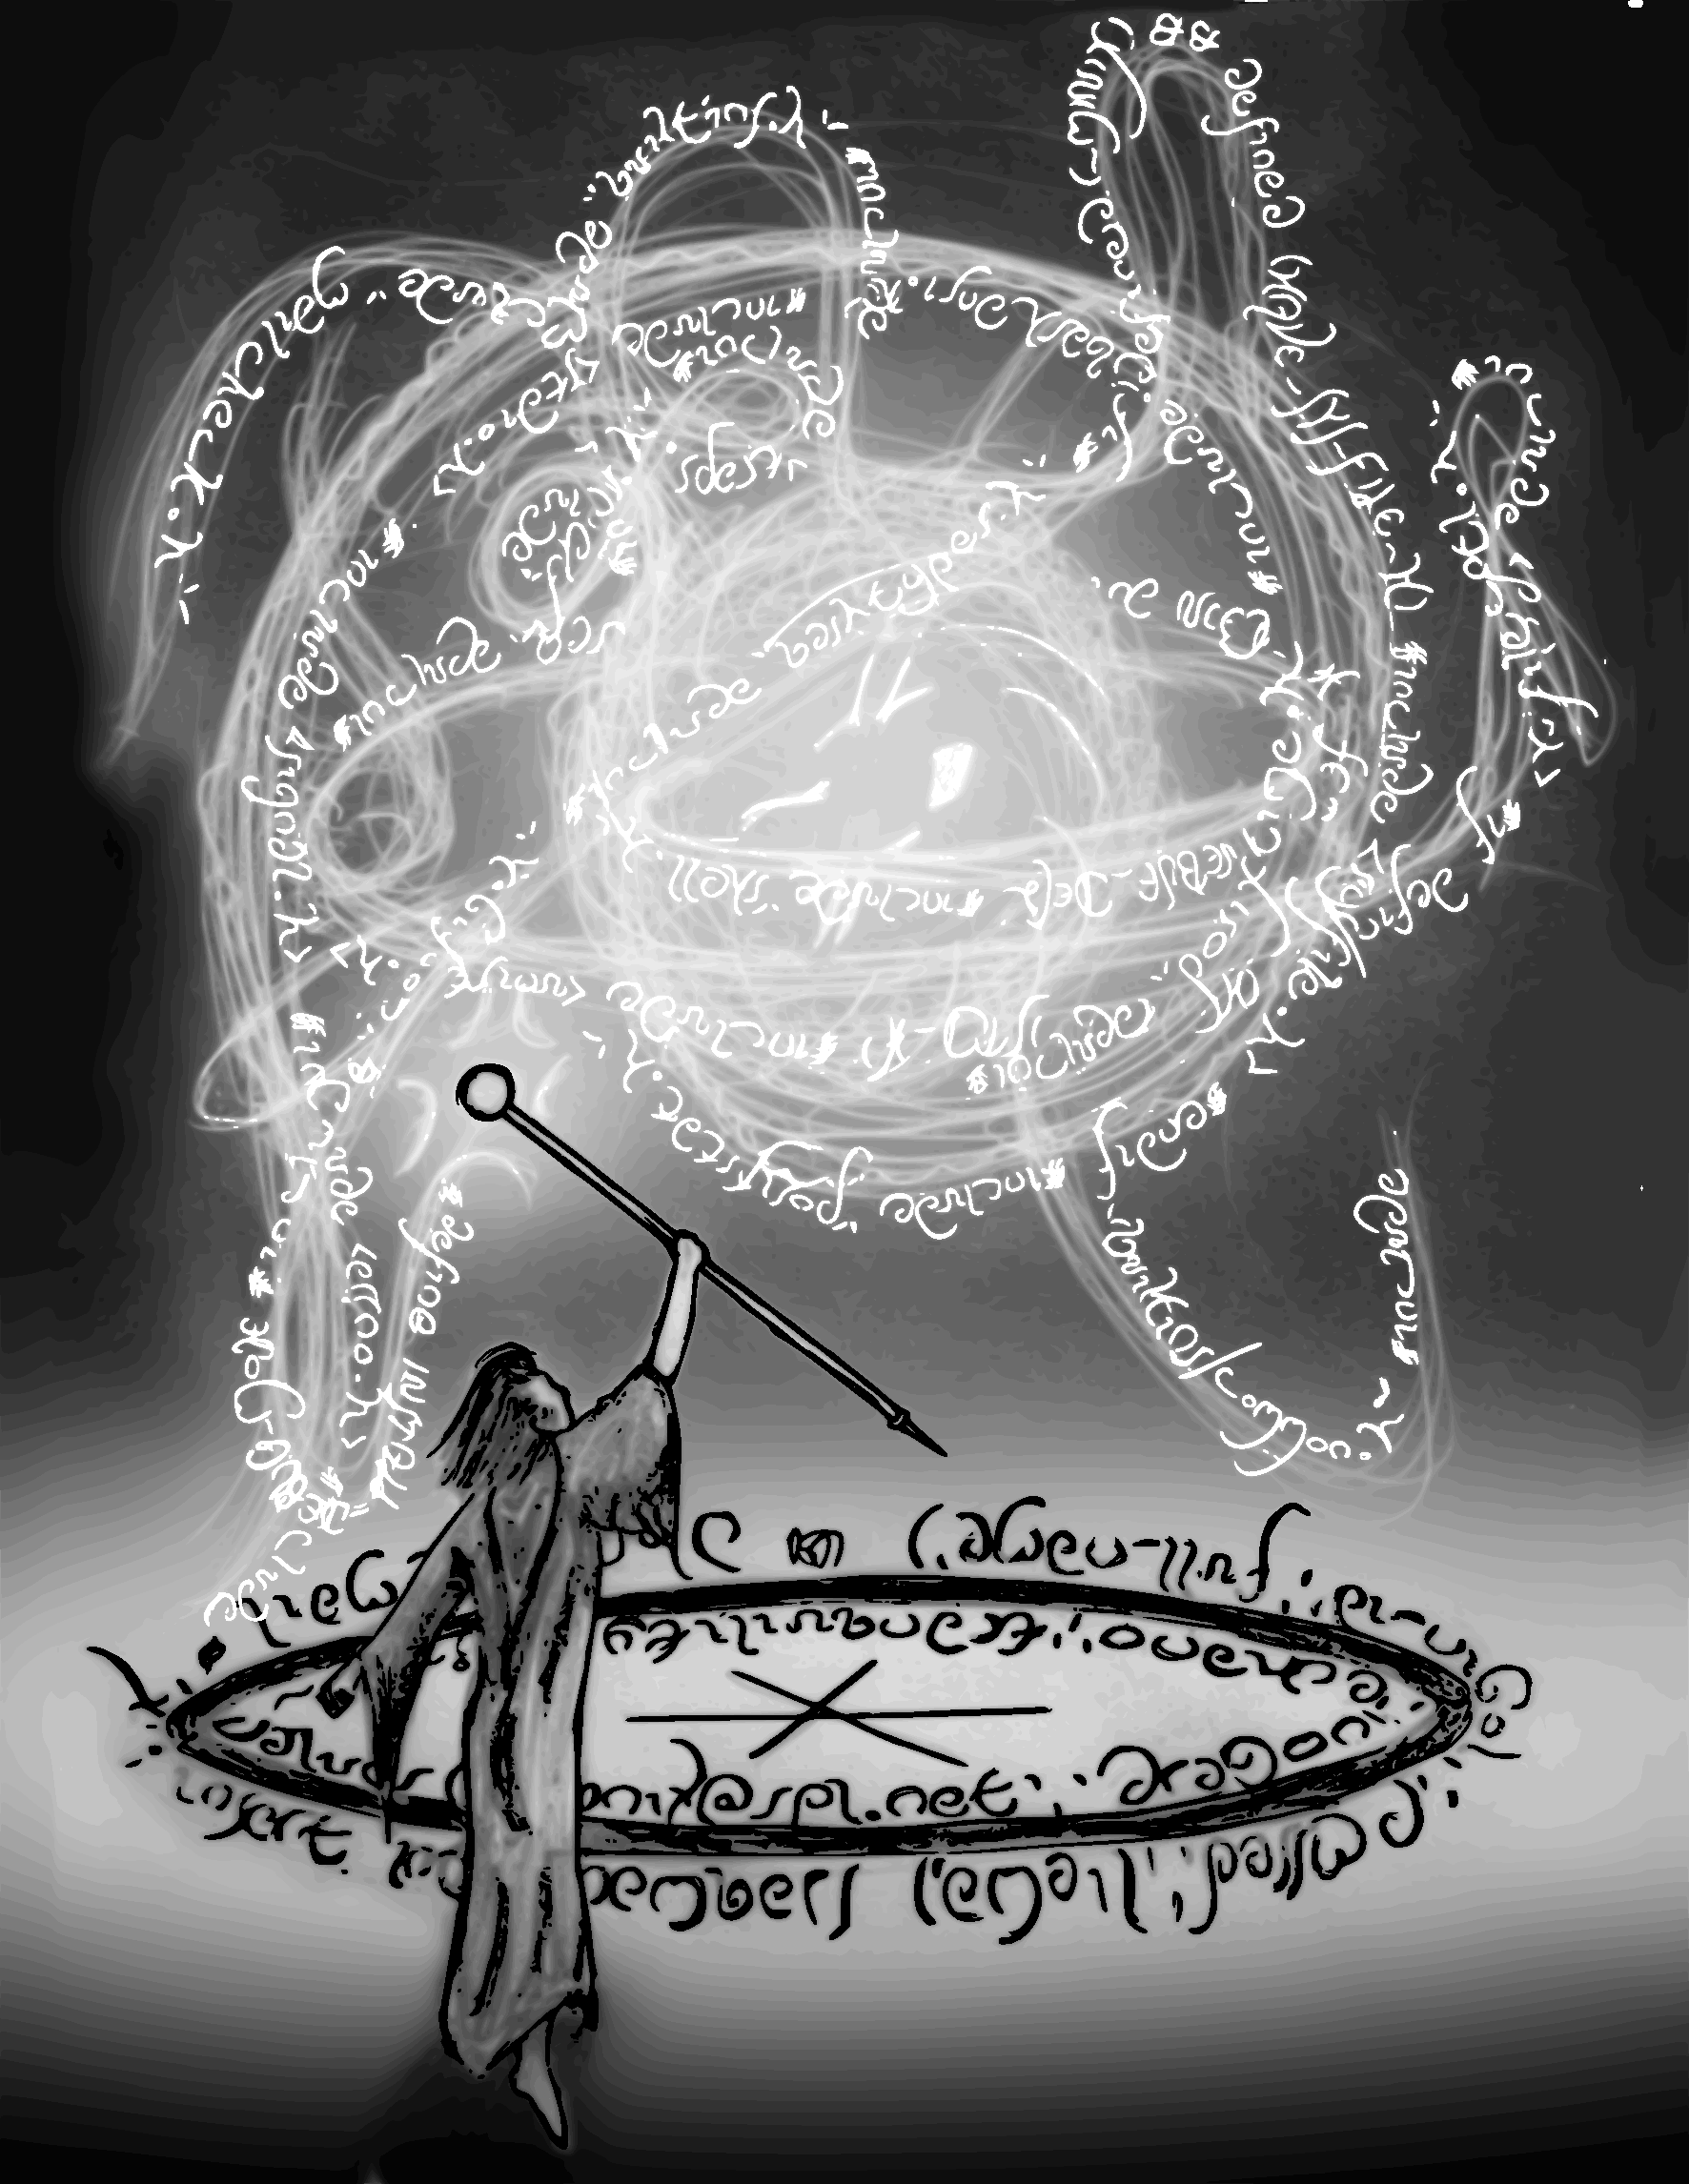
\includepdf[scale=1.007]{truedaemon.pdf}
